\documentclass[10pt,a4paper,journal,cspaper,compsoc]{IEEEtran}

% Some very useful LaTeX packages include:
% (uncomment the ones you want to load)

% *** CITATION PACKAGES ***
%
\ifCLASSOPTIONcompsoc
  % IEEE Computer Society needs nocompress option
  % requires cite.sty v4.0 or later (November 2003)
  \usepackage[nocompress]{cite}
\else
  % normal IEEE
  \usepackage{cite}
\fi
% cite.sty was written by Donald Arseneau
% V1.6 and later of IEEEtran pre-defines the format of the cite.sty package
% \cite{} output to follow that of IEEE. Loading the cite package will
% result in citation numbers being automatically sorted and properly
% "compressed/ranged". e.g., [1], [9], [2], [7], [5], [6] without using
% cite.sty will become [1], [2], [5]--[7], [9] using cite.sty. cite.sty's
% \cite will automatically add leading space, if needed. Use cite.sty's
% noadjust option (cite.sty V3.8 and later) if you want to turn this off.
% cite.sty is already installed on most LaTeX systems. Be sure and use
% version 4.0 (2003-05-27) and later if using hyperref.sty. cite.sty does
% not currently provide for hyperlinked citations.
% The latest version can be obtained at:
% http://www.ctan.org/tex-archive/macros/latex/contrib/cite/
% The documentation is contained in the cite.sty file itself.
%
% Note that some packages require special options to format as the Computer
% Society requires. In particular, Computer Society  papers do not use
% compressed citation ranges as is done in typical IEEE papers
% (e.g., [1]-[4]). Instead, they list every citation separately in order
% (e.g., [1], [2], [3], [4]). To get the latter we need to load the cite
% package with the nocompress option which is supported by cite.sty v4.0
% and later. Note also the use of a CLASSOPTION conditional provided by
% IEEEtran.cls V1.7 and later.


% *** GRAPHICS RELATED PACKAGES ***
%
  \usepackage[pdftex]{graphicx}
  \graphicspath{{../Figures/}}
  \DeclareGraphicsExtensions{.pdf,.png}
  \usepackage{color}

% *** MATH PACKAGES ***
%
\usepackage[cmex10]{amsmath}
% A popular package from the American Mathematical Society that provides
% many useful and powerful commands for dealing with mathematics. If using
% it, be sure to load this package with the cmex10 option to ensure that
% only type 1 fonts will utilized at all point sizes. Without this option,
% it is possible that some math symbols, particularly those within
% footnotes, will be rendered in bitmap form which will result in a
% document that can not be IEEE Xplore compliant!
%
% Also, note that the amsmath package sets \interdisplaylinepenalty to 10000
% thus preventing page breaks from occurring within multiline equations. Use:
%\interdisplaylinepenalty=2500
% after loading amsmath to restore such page breaks as IEEEtran.cls normally
% does. amsmath.sty is already installed on most LaTeX systems. The latest
% version and documentation can be obtained at:
% http://www.ctan.org/tex-archive/macros/latex/required/amslatex/math/

%\usepackage{amssymb}%............................ AMS Symbol fonts



% *** SPECIALIZED LIST PACKAGES ***
%
%\usepackage{algorithmic}
% algorithmic.sty was written by Peter Williams and Rogerio Brito.
% This package provides an algorithmic environment for describing algorithms.
% You can use the algorithmic environment in-text or within a figure
% environment to provide for a floating algorithm. Do NOT use the algorithm
% floating environment provided by algorithm.sty (by the same authors) or
% algorithm2e.sty (by Christophe Fiorio) as IEEE does not use dedicated
% algorithm float types and packages that provide these will not provide
% correct IEEE style captions. The latest version and documentation of
% algorithmic.sty can be obtained at:
% http://www.ctan.org/tex-archive/macros/latex/contrib/algorithms/
% There is also a support site at:
% http://algorithms.berlios.de/index.html
% Also of interest may be the (relatively newer and more customizable)
% algorithmicx.sty package by Szasz Janos:
% http://www.ctan.org/tex-archive/macros/latex/contrib/algorithmicx/

% *** ALIGNMENT PACKAGES ***
%
\usepackage{array}
% Frank Mittelbach's and David Carlisle's array.sty patches and improves
% the standard LaTeX2e array and tabular environments to provide better
% appearance and additional user controls. As the default LaTeX2e table
% generation code is lacking to the point of almost being broken with
% respect to the quality of the end results, all users are strongly
% advised to use an enhanced (at the very least that provided by array.sty)
% set of table tools. array.sty is already installed on most systems. The
% latest version and documentation can be obtained at:
% http://www.ctan.org/tex-archive/macros/latex/required/tools/


\usepackage{mdwmath}
\usepackage{mdwtab}
% Also highly recommended is Mark Wooding's extremely powerful MDW tools,
% especially mdwmath.sty and mdwtab.sty which are used to format equations
% and tables, respectively. The MDWtools set is already installed on most
% LaTeX systems. The lastest version and documentation is available at:
% http://www.ctan.org/tex-archive/macros/latex/contrib/mdwtools/

% IEEEtran contains the IEEEeqnarray family of commands that can be used to
% generate multiline equations as well as matrices, tables, etc., of high
% quality.

% *** SUBFIGURE PACKAGES ***
\ifCLASSOPTIONcompsoc
  \usepackage[caption=false,font=normalsize,labelfont=sf,textfont=sf]{subfig}
\else
  \usepackage[caption=false,font=footnotesize]{subfig}
\fi

%Setting captions to centered (Not IEEE journal standard)
%\makeatletter
%\long\def\@makecaption#1#2{\ifx\@captype\@IEEEtablestring%
%\footnotesize\begin{center}{\normalfont\footnotesize #1}\\
%{\normalfont\footnotesize\scshape #2}\end{center}%
%\@IEEEtablecaptionsepspace
%\else
%\@IEEEfigurecaptionsepspace
%\setbox\@tempboxa\hbox{\normalfont\footnotesize {#1.}~~ #2}%
%\ifdim \wd\@tempboxa >\hsize%
%\setbox\@tempboxa\hbox{\normalfont\footnotesize {#1.}~~ }%
%\parbox[t]{\hsize}{\normalfont\footnotesize \noindent\unhbox\@tempboxa#2}%
%\else
%\hbox to\hsize{\normalfont\footnotesize\hfil\box\@tempboxa\hfil}\fi\fi}
%\makeatother


% *** FLOAT PACKAGES ***
%
\usepackage{fixltx2e}
% fixltx2e, the successor to the earlier fix2col.sty, was written by
% Frank Mittelbach and David Carlisle. This package corrects a few problems
% in the LaTeX2e kernel, the most notable of which is that in current
% LaTeX2e releases, the ordering of single and double column floats is not
% guaranteed to be preserved. Thus, an unpatched LaTeX2e can allow a
% single column figure to be placed prior to an earlier double column
% figure. The latest version and documentation can be found at:
% http://www.ctan.org/tex-archive/macros/latex/base/

% *** PDF, URL AND HYPERLINK PACKAGES ***
%
\usepackage{url}

\usepackage{sistyle}
    \SIstyle{S-Africa}
    \SIunitspace{{\cdot}}
    \SIunitdot{{\cdot}}

% generate nice bookmarks and hyperrefs when exporting to pdf and dvi (screen version):
\usepackage[a4paper,plainpages=false,colorlinks,linktocpage,bookmarks=true,bookmarksopen=false]{hyperref}
% use this for printing only (no color, print version):
%\usepackage[a4paper,plainpages=false,colorlinks=false,linktocpage,bookmarks=true,bookmarksopen=false]{hyperref}

% correct bad hyphenation here
\hyphenation{op-tical net-works semi-conduc-tor}

%List of acronyms used in text
 \usepackage{acronym}%.......................... Acronym package to handle acronyms in text

\acrodef{MMOG}{Massively Multiplayer Online Game}
\acrodef{MMORPG}{Massively Multiplayer Online Role Playing Game}
\acrodef{WoW}{World of Warcraft}
\acrodef{MUD}{Multi-User Dungeon}
\acrodef{PvP}{Player-versus-Player}
\acrodef{P2P}{Peer-to-Peer}
\acrodef{CS}[C/S]{Client/Server}
\acrodef{CMS}[C/MS]{Client/Multi-Server}
\acrodef{NPC}{Non-Player Character}
\acrodef{aoi}[AoI]{Area of Interest}
\acrodef{alm}[ALM]{Application Level Multicast}
\acrodef{ui}[UI]{User Interface}
\acrodef{DHT}{Distributed Hash Table}

\begin{document}

%
% paper title
\title{A Survey of State Persistency in Peer-to-Peer Massively Multiplayer Online Games}

\author{John~S.~Gilmore~and~Herman~A.~Engelbrecht% <-this % stops a space
\IEEEcompsocitemizethanks{\IEEEcompsocthanksitem J.S. Gilmore and H.A. Engelbrecht are with the MIH Media Laboratory at the Department of Electrical
and Electronic Engineering, Stellenbosch University, Stellenbosch, South Africa.\protect\\
% note need leading \protect in front of \\ to get a newline within \thanks as
% \\ is fragile and will error, could use \hfil\break instead.
E-mail: jgilmore@ml.sun.ac.za and hebrecht@sun.ac.za}% <-this % stops a space
\thanks{}}

% The paper headers
\markboth{Draft Submission to the Journal of Parallel and Distributed Systems, July~2010}%
{Draft Submission to the Journal of Parallel and Distributed Systems, July~2010}
% The only time the second header will appear is for the odd numbered pages
% after the title page when using the twoside option.

% The publisher's ID mark at the bottom of the page is less important with
% Computer Society journal papers as those publications place the marks
% outside of the main text columns and, therefore, unlike regular IEEE
% journals, the available text space is not reduced by their presence.
% If you want to put a publisher's ID mark on the page you can do it like
% this:
%\IEEEpubid{0000--0000/00\$00.00~\copyright~2007 IEEE}
% or like this to get the Computer Society new two part style.
%\IEEEpubid{\makebox[\columnwidth]{\hfill 0000--0000/00/\$00.00~\copyright~2007 IEEE}%
%\hspace{\columnsep}\makebox[\columnwidth]{Published by the IEEE Computer Society\hfill}}
% Remember, if you use this you must call \IEEEpubidadjcol in the second
% column for its text to clear the IEEEpubid mark (Computer Society jorunal
% papers don't need this extra clearance.)

% for Computer Society papers, we must declare the abstract and index terms
% PRIOR to the title within the \IEEEcompsoctitleabstractindextext IEEEtran
% command as these need to go into the title area created by \maketitle.
\IEEEcompsoctitleabstractindextext{%
\begin{abstract}
%\boldmath
Recently, there has been a drive to move away from a Client/Server approach to Massively Multiplayer Online Games to a Peer-to-Peer
approach. This can been seen when looking at the number of articles published on Peer-to-Peer systems compared to those published on Client/Server
systems. This proposal discusses the different architectures currently in use and discusses the key challenges that a move to Peer-to-Peer presents.
From the discussion, a novel architecture based on groups of players is proposed in an attempts to exploit the flocking behaviour of players. Focus
is also placed on state persistency and a hybrid state consistency model is presented to deal with persistency in games. The model distinguishes
between ephemeral and persistent data in an attempt to improve the responsiveness of the storage. The model makes use of both overlay storage as well
as distance based storage to achieve these ends.
\end{abstract}
% IEEEtran.cls defaults to using nonbold math in the Abstract.
% This preserves the distinction between vectors and scalars. However,
% if the journal you are submitting to favors bold math in the abstract,
% then you can use LaTeX's standard command \boldmath at the very start
% of the abstract to achieve this. Many IEEE journals frown on math
% in the abstract anyway. In particular, the Computer Society does
% not want either math or citations to appear in the abstract.

% Note that keywords are not normally used for peer review papers.
\begin{IEEEkeywords}
A.1.0 [\textbf{Introductory and Survey}], J.8.d [\textbf{Internet Applications}]: Distributed file systems, J.8.g [\textbf{Internet Applications}]:
Games
\end{IEEEkeywords}}

% make the title area
\maketitle

% To allow for easy dual compilation without having to reenter the
% abstract/keywords data, the \IEEEcompsoctitleabstractindextext text will
% not be used in maketitle, but will appear (i.e., to be "transported")
% here as \IEEEdisplaynotcompsoctitleabstractindextext when compsoc mode
% is not selected <OR> if conference mode is selected - because compsoc
% conference papers position the abstract like regular (non-compsoc)
% papers do!
\IEEEdisplaynotcompsoctitleabstractindextext
% \IEEEdisplaynotcompsoctitleabstractindextext has no effect when using
% compsoc under a non-conference mode.

% For peer review papers, you can put extra information on the cover
% page as needed:
% \ifCLASSOPTIONpeerreview
% \begin{center} \bfseries EDICS Category: 3-BBND \end{center}
% \fi
%
% For peerreview papers, this IEEEtran command inserts a page break and
% creates the second title. It will be ignored for other modes.
\IEEEpeerreviewmaketitle

%\section{Introduction}
% Computer Society journal papers do something a tad strange with the very
% first section heading (almost always called "Introduction"). They place it
% ABOVE the main text! IEEEtran.cls currently does not do this for you.
% However, You can achieve this effect by making LaTeX jump through some
% hoops via something like:
%
\ifCLASSOPTIONcompsoc
  \noindent\raisebox{2\baselineskip}[0pt][0pt]%
  {\parbox{\columnwidth}{\section{Introduction}\label{sec:introduction}%
  \global\everypar=\everypar}}%
  \vspace{-1\baselineskip}\vspace{-\parskip}\par
\else
  \section{Introduction}\label{sec:introduction}\par
\fi
%
% Admittedly, this is a hack and may well be fragile, but seems to do the
% trick for me. Note the need to keep any \label that may be used right
% after \section in the above as the hack puts \section within a raised box.

% The very first letter is a 2 line initial drop letter followed
% by the rest of the first word in caps (small caps for compsoc).
%
% form to use if the first word consists of a single letter:
% \IEEEPARstart{A}{demo} file is ....
%
% form to use if you need the single drop letter followed by
% normal text (unknown if ever used by IEEE):
% \IEEEPARstart{A}{}demo file is ....
%
% Some journals put the first two words in caps:
% \IEEEPARstart{T}{his demo} file is ....
%
\IEEEPARstart{P}{eer-to-Peer (P2P)} Massively Multiplayer Online Games (MMOGs) have received a significant amount of attention from the research
community over the past years. Since the first publication on the subject by Knutssonn et al. \cite{knutsson_p2p_first}, the three areas of Interest
Management, Game Event Dissemination and Security, have received much attention from the research community, but the area of Game State Persistency
has remained mostly unexplored.

Interest Management determines how player actions are filtered to ensure that players only receive actions relevant to them, which reduces the
bandwidth requirements of the system. Game Event Dissemination entails how these events are then sent to various players. Security ensures that the
system is not affected by the activity of malicious peers.

Game State Persistency entails storing persistent game data in a distributed way over the the P2P network. Part of an MMOG is ensuring low latency,
consistent data persistency of all game data. Player data, in-game object states and NPC states should all be stored and in a P2P system, these
states should be stored in a distributed way, as no central object database is present to provide this storage.

This paper classifies the techniques used in documented P2P MMOG architectures and discusses the advantages and disadvantages of the different types
of storage. To the best of our knowledge, such a classification has not been undertaken in the literature, where a focus is placed specifically on
state persistency in P2P MMOGs. As the field of P2P MMOGs is a growing one, it is believed that a comprehensive survey of persistency techniques is
required to act as a basis for further research into this field.

The survey will firstly present an overview of classic models used in Client/Server (C/S) and P2P multiplayer games. P2P MMOG state persistency
techniques are then classified in terms of the type of storage they provide and key challenges are defined by which the performance of these storages
may be measured. The three identified types of storage are then described and evaluated according to the key challenges, which is followed by a
discussion of possible measurable metrics by which the performance of a state persistency model might be measured.


Section \ref{classic_models} details how state persistency is handled in P2P, C/S and Client/Multi-Server (C/MS) systems employed in multiplayer
games today.
%
Section \ref{p2p_mmog_models} details how state persistency is implemented in P2P MMOGs by defining five key challenges and then discussing three
approaches according to the identified challenges.
%
Section \ref{eval_crit} attempts to define measurable metrics according to the key challenges to enable the performance of different state
persistency models to be compared.


\section{Classic consistency models}
\label{classic_models}

A consistency model is based on the network architecture, but deals with how data are stored and distributed throughout the system. The consistency
model specifies on what type of nodes what types of data are stored and also how data consistency is ensured with multiple node requests.

To understand consistency models, some basic terms should first be understood. These terms are: ``event'', ``update'', ``game state'', ``game logic''
and ``game object''.

\emph{Events:} Events are generated by players and can be thought of as actions taken by players. These include casting a spell, using an item
    or walking.

\emph{Game Logic:} Game logic is applied to events to determine what updates should be applied to the game state. Game logic is thus a
    ``think'' function, which determines how the world should change as a result of an event. Another way to think about game logic is to see
    it as the game rules. A player casting a spell might cause another player's health to be reduced, her own health to be increased or a
    monster to spawn. When a player is walking, the logic will cause the player's position to update at the player's walking speed.

\emph{Update:} Game logic communicates how the world should change via game updates. Game updates are the incremental changes that specify how
    the current state should change.

\emph{Game State} The state of the game is the positions, health and all other attributes of all players, NPCs and game objects in the game
    world. Game state consists of a collection of game objects. An NPC as well as an immutable plant are both examples of game objects that
    together make up the game state.

\emph{Game objects:} When discussing how to segment game state, it is sometimes easier to speak in terms of game objects, since they are
    separable. For the purposes of this work, game objects are objects with both state and logic, which means they consume both storage
    space, as well as CPU power. Game objects can also produce events, which should be sent to other objects. When this definition is used,
    NPC objects may be classified as a specific type of a game object, which forms part of the global game state. The question of NPC hosting
    then also becomes a question of state persistency.



\subsection{P2P and C/S consistency models}
\label{p2p_cs_models}

As an introduction to consistency models, an overview of the two common models, currently used in computer games will be described. The models used
in P2P MMOGs are all permutations of these two basic models. The two models are based on the two different network models. These are the P2P-based
model, also called the event-based model \cite{p2p_cm_aoe}, and the Client/Server-based model, also called update-based model
\cite{unreal_networking}.

\subsubsection{Event-based}

\begin{figure*}[htbp]
\centering
\subfloat[Update-based (peer-to-peer)]{\label{fig_p2p_cm}
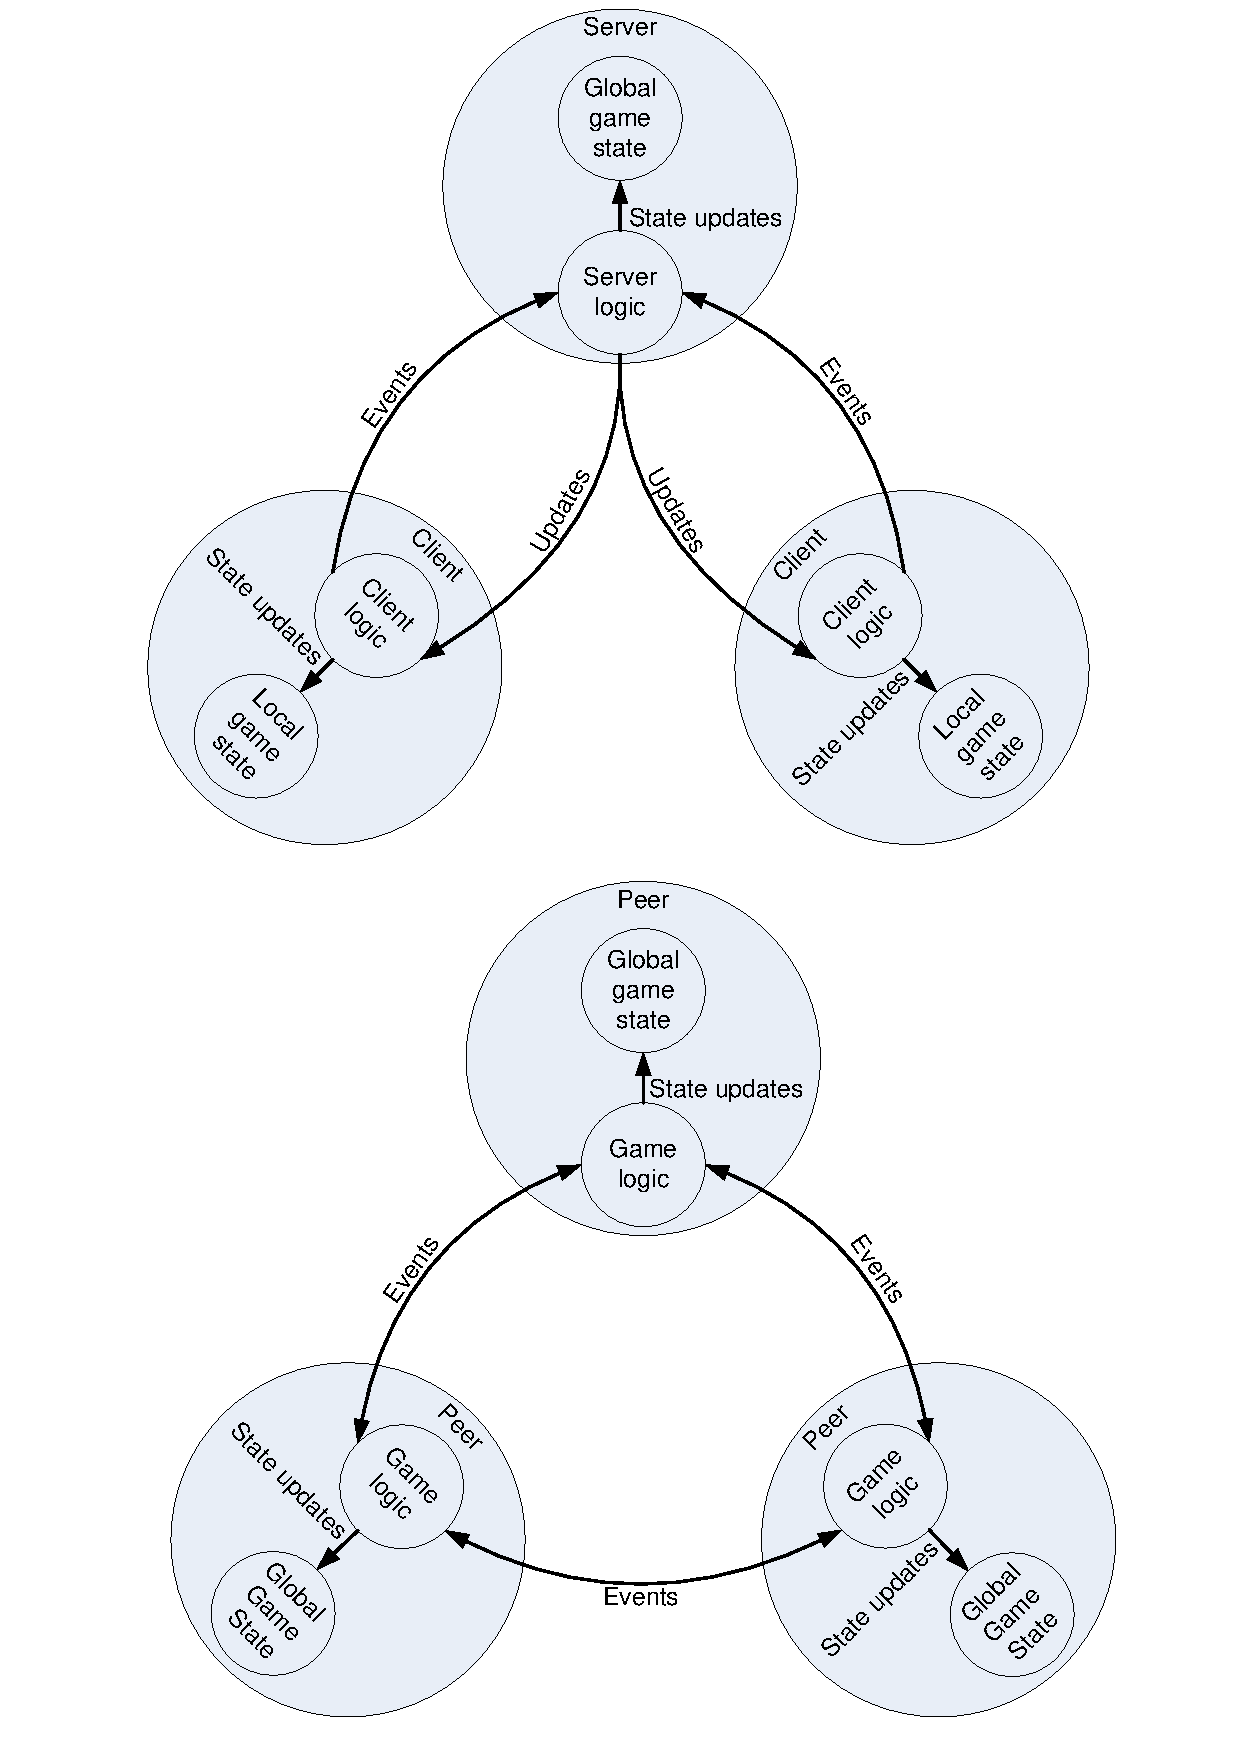
\includegraphics[clip=true, viewport= 2.5cm 0.5cm 19cm 15cm, width=\columnwidth]{CS_P2P_CMs}}
 \subfloat[Event-based (client/server)]{\label{fig_cs_cm}
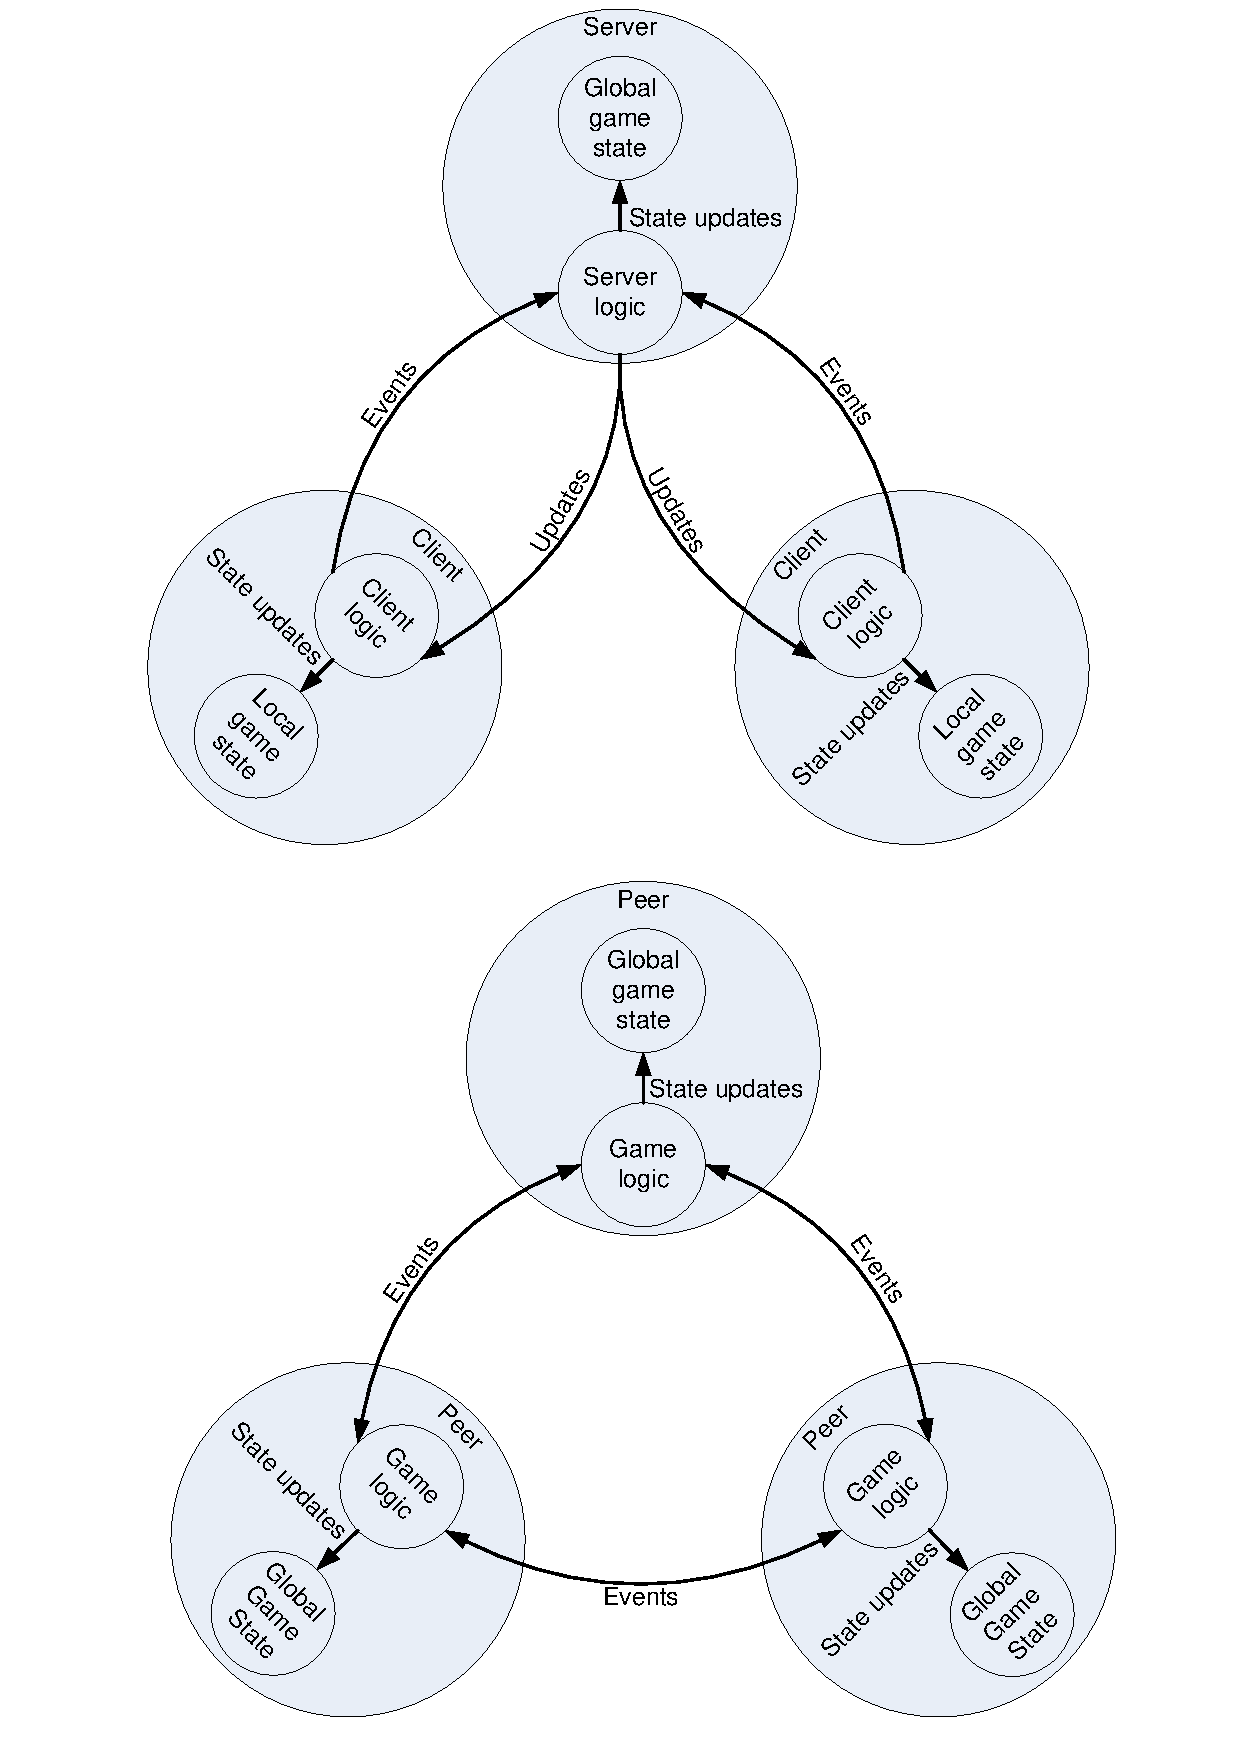
\includegraphics[clip=true, viewport= 2.5cm 15cm 19cm 30cm, width=\columnwidth]{CS_P2P_CMs}}
\caption{Consistency models}
\end{figure*}
%
Figure \ref{fig_p2p_cm} shows the P2P model. In this model the complete game state is stored on each peer. Any event that a peer generates is sent to
all other peers. These events are used as inputs to the game logic, which creates updates, which are used to update the global game state at each
peer.

It is at this level that consistency becomes important. The order in which updates are received should be the same for all peers, otherwise the game
states of different peers may become inconsistent. Usually some kind of lockstep technique is used to solve this issue \cite{pessimistic_lock_step}.
The issue with lockstep is that it reduces the latency to twice that of the peer with the highest latency. Various techniques have been proposed that
improves the latency by introducing some deadline before which all events should be submitted \cite{cheat_proof_event_ordering}. This, however, makes
it impossible for a player with a high latency to play the game with anyone other than from her own continent.

The issue with the event-based model is that it is not scalable, since all peers should connect to all other peers and every event is transmitted to
everyone. This means that as $N$, the number of peers in the network, increases, the amount of traffic increases with a factor of $N^2$. The security
issues of the P2P networking model, on which this consistency model is based, are also present. Slowdown is also experienced by all players if one
player's latency is below par, since the lockstep mechanism has to wait for all events to be received for that round to conclude.

\subsubsection{Update-based}
An alternative to the event-based model is the update-based model, shown in Figure \ref{fig_cs_cm}. This model is based on the Client/Server
networking model. An authoritative global game state is housed on the server and a non-authoritative local game state is housed on all clients for
display purposes. No real game logic is housed at the clients, only on the server. All clients send events to the server, which applies the game
logic and sends updates to the clients, while also updating its own game state.

This approach greatly assists with security, as clients cannot influence the state of any other clients and every client's state depends on updates
received from the server. The server state is also termed authoritative, because if there is a conflict, the server state is always the state to
which the system is expected to return. All the security advantages of the \ac{CS} model also apply to this consistency model. Another reason why the
event based model is successful is because it is more scalable then the pure P2P model. More hardware can be used to build a more powerful server,
which can handle more clients. This is however very costly as discussed in Section \ref{classic_network_models}.

\subsection{Client/Multi-Server consistency models}
\label{cms_models}

%Should I add diagrams here?

Apart from the two classic models, there are also models based on the \ac{CMS} network model, which are: shard-based, replication-based, object-based
and zone-based \cite{Hu_voronoi_IM}.

\subsubsection{Sharding}
Sony introduced the first consistency method for a \ac{CMS} network in Everquest, where copies of the game world ran on different servers and players
connected to one of these servers \cite{engineering_everquest}. Sony termed this method: ``Sharding''. Clients are not able to interact or
communicate with players on other shards, which reduces game immersion. This method does, however, allow for a more scalable system as maximum load
is fixed. Players are not able to enter a shard if that shard has reached it capacity. This has in the past caused unhappiness amongst players, since
popular shards could be difficult to log in to. Players are also reluctant to move to a new shard, because a lot of time is invested in their
characters in their ``home'' shard. Sharding doesn't allocate resources efficiently, as one shard may be overpopulated while another is
underpopulated. There is no way to dynamically distribute the available resources from one shard to another. For all practical purposes, this
approach is still merely a \ac{CS} approach, with players forced into a specific \ac{CS} environment.

\subsubsection{Replication-based}
%Redundant
The replication-based model is very similar to sharding, with the difference that all servers share the same duplicated game state. Each server
contains the global game state and clients connect to any one of these servers (mirror-servers \cite{mirrored_server}) or through a load distribution
algorithm to a server (proxy-servers \cite{proxy_server_dist}). Each server handles all actions from clients and updates its own database. The
servers in turn send updates to each other over a high quality link, such as fibre, to maintain database consistency at high speeds. The problem with
this system is that the world is never truly consistent and that there are no optimally chosen inconsistency obfuscation boundaries. In other words,
two players standing next to each other in the virtual world, might be on different servers and, therefore, experience two slightly different worlds.

\subsubsection{Object-based}
%Object based
The object-based method distributes all in-game objects amongst the servers \cite{object_based_consistency1}, \cite{object_based_consistency2},
\cite{object_based_consistency3}. For an MMOG, most of these objects are expected to be players objects. The advantage of this method is that the
system load is fixed for a certain player population and that the load is equally distributed amongst all servers. This allows for more accurate
prediction and provisioning  of required resources, but still does not handle transient loads well. Another issue is inter-server communications for
this architecture. The inter-server communications are random and also much more than the inter-server communications for a region based system. The
reason for this is that the amount of player interaction increases with a decrease in the distance between the players. Players playing together move
together, chat and interact with \acp{NPC} together. For a region based model, all player-neighbour interactions remain local to the server.

\subsubsection{Zone/Region-based}
%Zone-based
The zone-based method divides the virtual world into zones or regions, which are hosted on different servers \cite{zone_based_stat},
\cite{zone_based_dyn}. Busy regions are hosted on their own servers, while multiple quiet regions are hosted on a single server. This is termed the
static region approach \cite{zone_based_stat}. The issue of the static region approach is that it does not scale well when one region is suddenly
populated with players. This type of behaviour happens quite regularly and is known as flocking \cite{flocking}. When players find something of
interest in a region, many players will flock to that region. In-game events and festivals are also becoming popular and these events also cause
flocking to the region where the event is held. The solution to these effects have been over provisioning of resources to handle peak loads, which
suffers from the disadvantages discussed above. Also, if the load changes, the server has to be brought off-line in order to balance the regions.
Dynamic regions are being investigated, where regions can be dynamically shifted from one server to another, in order to balance load
\cite{zone_based_dyn}. This approach adds overhead and significant complexity with regards to the migration of the data and the handling of player
actions while the data are in transit.

\section{P2P MMOG consistency models}
\label{p2p_mmog_models}

\subsection{Key Challenges}
\label{key_challenges_cm}

%Consistency issues
The key challenges related to P2P MMOG consistency models identified during this literature study were: reliability, responsiveness, security,
fairness and consistency.


\emph{Reliability:} For the storage to be reliable, it must not be possible for data to be lost, and stored data should always be available when a
    node requests it.

\emph{Responsiveness:} To ensure system responsiveness, data must be stored or retrieved in real-time. With real-time, it is meant that data
    should be available within a certain time frame that would ensure correct functionality of the MMOG requiring it. The variance in times when
    data become available should also be small.

\emph{Security:} The storing system should store data securely. It should not be possible for data to be altered in ways that are inconsistent
    with the game rules. It should also be possible to identify nodes that alter the data in this malicious way. This also adds the requirement
    that nodes should be authenticated in the storage system and that only authorised nodes should be able to alter data.

\emph{Fairness:} Ensuring fairness in the system means distributing load evenly according to the abilities of individual nodes. This ensures that
    not only a small number of nodes provide all system resources required for the system to function, but that all nodes contribute what they
    can, in order to support the system.

\emph{Consistency:} The consistency requirement specifies that nodes should perceive the game world as the same. This is intentionally a vague
    requirement, as it is believed that the stricter requirement of the game world actually being the same is too strong. When two players are
    playing together, they should perceive the world exactly the same way. If, for example, one player perceives a monster and starts to attack
    it, while the other player sees nothing, the game experience of both will degrade. As another example, if there is a damsel in distress in a
    tower for a player that visits the tower, but no damsel for a player that does not enter the tower, the game experience would not degrade.
    This is because the player not in the tower does not have to know about the damsel. From these two examples, the reason for state persistency
    based on perception, rather than reality is shown.


All state persistency models will be reviewed with these issues in mind.

\subsection{Overview of approaches}
\label{p2p_mmog_cm_overview}

%Overview of three approaches
Very little work has been done on state persistency for P2P MMOGs. Generally three approaches have been identified for state persistency: super peer
storage \cite{knutsson_p2p_first}, overlay storage \cite{Douglas05enablingmassively}, \cite{using_freenet_storage}, \cite{Fan_phd},
\cite{past_storage_focus} and distance-based storage \cite{Buyukkaya_voronoi_state_management}, \cite{Hu_voronoi_IM}, \cite{colyseus_distance_based}.
Hybrid techniques, distinguishing permanent data from ephemeral data have also been proposed \cite{zoned_federation}, \cite{hybrid_storage1}.

\begin{table*}[htbp]
\centering
\begin{tabular}{|r|c|c|c|c|c|}
\hline
Storage type & Reliability & Responsiveness & Security & Fairness & Consistency\\
\hline
Region-based Super Peer & Medium & High & Low & Low & High\\
Overlay & High & Low & Medium & High & Low\\
Region-based Super Peer/Overlay & High & High & Low & Low & High\\
Distance-based & Low & High & Low & High & High\\
\hline
\end{tabular}
\caption{Differences between storage mechanisms} \label{tab_storage}
\end{table*}
%
Table \ref{tab_storage} presents a summary of how current storage systems handle the five key issues identified. From this table it can be seen that
no one storage mechanism has fully addressed all the identified issues. What is also shown is that architectures that differentiate between different
types of data, are theoretically better suited to the MMOG application. The example of such an architecture is the hybrid architecture, which also
seems to fare best, when compared to other storage techniques.

\subsection{Super peer storage}

%Super peer storage - description
Super peer storage relies on the super peer storing all relevant information in its domain. An example of this is in \cite{knutsson_p2p_first}, where
the world is segmented into regions and super peers act as regional servers to all peers in their region. Each super peer handles all game logic and
distributes updates to all peers in its region. The super peer also handles state persistency for its region, hosting NPCs, objects and persistent
player data.

\begin{figure*}[htbp]
 \centering
 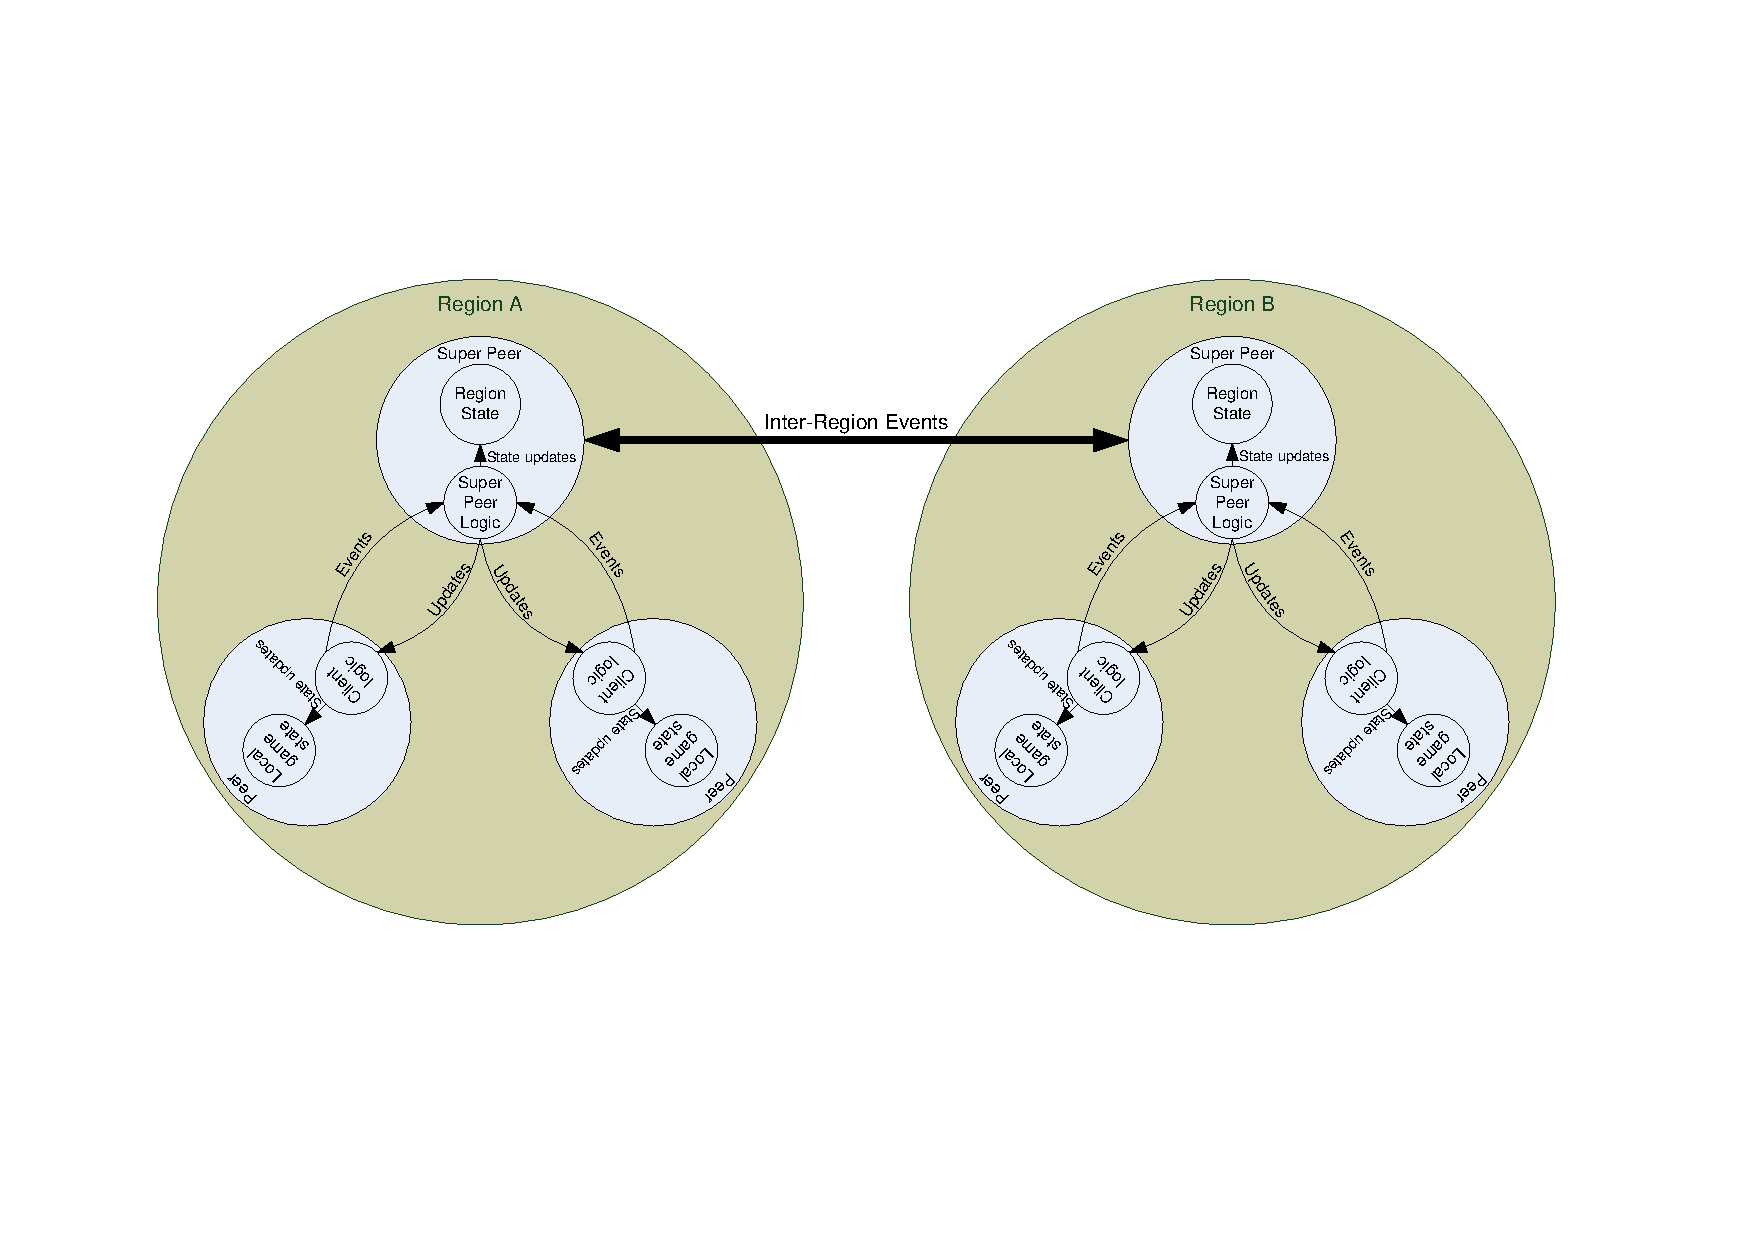
\includegraphics[clip=true, viewport=2cm 5cm 27cm 16.5cm, width=\textwidth]{region_based_CS_CM}
 \caption{Region-based Client/Server consistency model}
 \label{fig_cs_region_cm}
\end{figure*}
%
The consistency model for this approach is depicted in Figure \ref{fig_cs_region_cm}. One can see that this approach is modelled on the update based
model, but segmented into separate regions. The role of the server is here fulfilled by a super peer, which is a peer that is selected in some
logical way, from the available set of peers and then promoted. Server selection in itself is a complex topic that has to deal with determining
whether a peer has sufficient resources available and also whether the peer is trustworthy.

Each super peer in this model houses the complete region state as shown. Super peers also house the real game logic. Clients in the region only house
copies of the regional objects and some client logic to update the local copies of objects housed. Like the \ac{CS} model, clients only send events
to super peers, where super peers apply the game logic and send state updates to clients.

\subsubsection{Fairness}
%Super peer storage - issues
The super peer storage model has many potential issues. Overloading of the super peer is one. A super peer could be relatively easily overloaded if a
region becomes too crowded, since a super peer is merely the computer of some player in the game and not a specialised server machine. The question
of fairness also arises. The idea of a P2P MMOG model is that all peers share resources. With this model, peers with extra resources are expected to
donate these resources for the good of all. Players might consider it unfair, when they are constantly expected to donate resources, some of which
they might have to pay for.

\subsubsection{Reliability}
Another issue is reliability. In a P2P system, with a high rate of churn, players are expected to constantly leave and join the network. Because of
this reality, redundancy mechanisms have to be developed that would ensure state data are always available, even when a super node leaves the
network. It is possible to solve these issues by having redundant super peers in each region, that take over hosting responsibility if the main super
peer leaves. One method by which redundant region coordinators are maintained in \cite{knutsson_p2p_first}, is to create backup coordinators on peers
with IDs closest to the current coordinator. This means that if the main coordinator fails, all data will automatically be routed to the backup,
because of the feature of DHTs. It is important that the main and backup super peers always posses consistent states, even during a transition from
main to backup. Other schemes to support improved reliability deal with reputation mechanisms for super peers. Super peers that have more resources
and stay in the network longer are preferred during super peer selection, using reputation mechanisms \cite{fan_mediator_paper}.

\subsubsection{Security}
The third, and probably most important issue is that of security. If a single peer is allowed to house the player information of a large group of
players, it might become possible for such a peer to modify the data to suit his own ends. The issue is not only that modification of the data might
be possible, but also that it would not be possible for the cheating to be detected, because of no centralised logging. A scheme that would improve
the reliability of this systems has been proposed, where every event is also sent to the backup super peer of the region \cite{past_storage_focus}.
The main super peer responds with the update and the backup super peer responds with a hash of the update. A peer can then check whether the hashes
match to determine whether the data has been received correctly. A hash is not the state update itself, so will be much smaller, but the events that
have to be sent to all super peers will increase traffic in the network and bandwidth usage by peers.

\subsubsection{Responsiveness}
There are, however, also advantages to super peer storage. All data are stored on the super peer, which means that storing data is a low latency
operation. The regional state can be stored and retrieved at very high speeds, making the system very responsive. Data retrieval from such a storage
is also relatively fast; as fast as data retrieval from a server. Peers can request data from a super peer and the data can be returned to the peer
in one hop after transmission of the request. Super peers may, however, become overloaded with requests and thereby increase the latency of the
system.

\subsubsection{Consistency}
Super peer storage is always consistent, because event ordering is handled by a centralised super peer for each region. If events occur across region
boundaries, the super peer of the region in which the event was triggered will send a message to the super peer in the region affected by the event.
This is also an event that can be ordered, as the one super peer is handled as a normal peer for the consistency calculation.

\subsection{Overlay storage}
\label{overlay_storage}

%Overlay storage - description
\begin{figure*}[htbp]
 \centering
 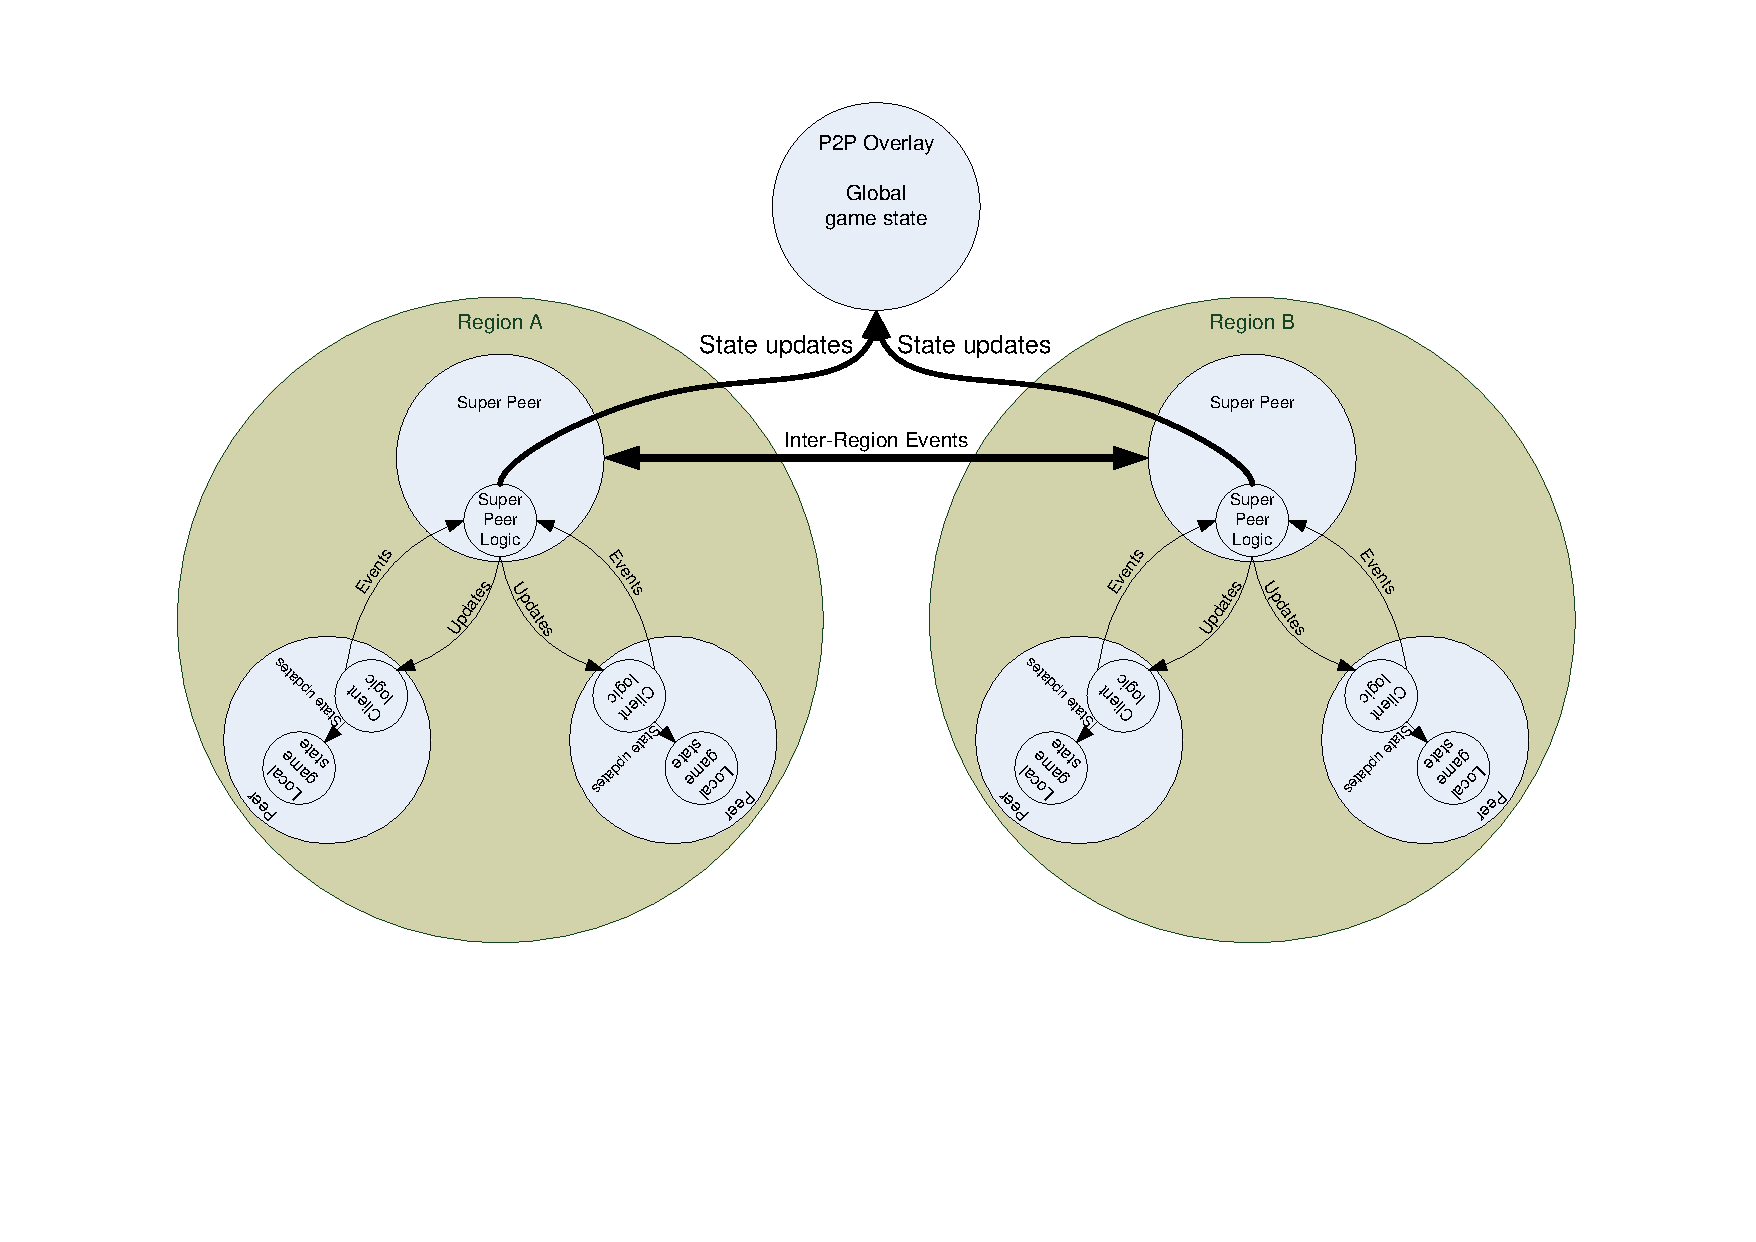
\includegraphics[clip=true, viewport=2cm 5cm 27cm 19.5cm, width=\textwidth]{region_based_CS_CM_P2PO}
 \caption{Region-based Client/Server with overlay consistency model}
 \label{fig_cs_region_o_cm}
\end{figure*}
%
Overlay storage, shown in Figure \ref{fig_cs_region_o_cm} entails using a distributed file storage system, which is based on a P2P overlay to host
objects. Figure \ref{fig_cs_region_o_cm} actually shows a type of Super Peer/Overlay hybrid storage implemented in \cite{zoned_federation}, but the
basic principles remain the same. The model depicted in Figure \ref{fig_cs_region_o_cm}, uses an overlay storage managed by regional super peers. The
reason for this management is to achieve state consistency. Although game state is always consistent in overlay storage, because of the inherent
consistency of DHTs, issues of serialisability can still occur \cite{zoned_federation}. In order for game states to remain consistent, events should
be serialisable. In the context of state consistency, this means that the order in which events are received at any peer, should be the same. This
cannot be ensured in this case, because there is no central entity that orders events and an update-based model is not used. If the order in which
events are processed are not the same, state inconsistencies may arise.

The world is divided into regions and so data stored for one region will have no effect on the sate of other regions. This can of course be debated,
but for global specific data a global ``region'' can be created. Super peers then act as servers that use their section of the overlay as their own
storage databases. Data consistency may be assured as all access to a region's data is controlled by that region's super peer. The Zoned Federation
model further uses local caching at super peers to achieve real-time access to data. Overlay storage is used as a backup mechanism to achieve data
persistency and redundancy.

%Overlay storage - reason
Overlay storage is a very popular storage method, currently used by most P2P MMOG architectures. This is believed to be more as a consequence of the
use of Scribe than any inherit benefit to P2P MMOGs \cite{past_storage_focus}. This is also the motivation used in Chapter 4 of \cite{Fan_phd}, where
the Mediator architecture is described. Scribe is an implementation of \ac{alm} that uses the Pastry overlay as the structure to send multicast
messages over \cite{scribe}. PAST is a distributed persistent storage implemented to use Pastry for routing data and requests for data. The reason
for using overlay storage in so many implementations seem to be merely the availability after using Scribe. The implementation of state persistency,
however, does not have to be linked with the event dissemination scheme. A P2P overlay may be used for event dissemination, and another method can be
used to ensure state persistency.

\subsubsection{Responsiveness}
%Overlay storage - issues
An evaluation of overlay storage also shows some issues when used for state persistency in MMOGs. The main issue with this mode of storage is summed
up by the creators of PAST: ``Finally, PAST is intended as an archival storage and content distribution utility and not as a general-purpose
filesystem. It is assumed that users interact primarily with a conventional filesystem, which acts as a local cache for files stored in PAST.''
\cite{storage_and_chaching_PAST}. This is not how the file system interaction occurs in MMOGs. For responsive MMOGs, a distributed file system is
required that allows for real-time file storage and retrieval.

The most significant issue with overlay storage is the delay incurred when storing and retrieving data. As data can be stored anywhere on the network
and the network is not fully connected, it takes $O(\log_{2^4}(N))$ hops on average to retrieve or store a data item using Pastry
\cite{storage_and_chaching_PAST}. Although this is a good order complexity for a routing algorithm in a large network, it is not sufficient to
support a real-time application. This latency issue is the same issue that is present in \ac{alm} as discussed in Section
\ref{proposed_architecture}.

\subsubsection{Consistency}
Different types of overlays have different advantages and disadvantages. A pure overlay-based storage scheme performs very badly. The scheme is
inconsistent, because there is no way to synchronise the order of events amongst nodes, which leads to inconsistent states.

\subsubsection{Security}
This model does have better security than the super peer storage model as data are distributed amongst all peers and redundancy and quorum techniques
can be implemented to ensure that files are retrieved with a high level of security. Why the security is rated as average is not because a real lack
of security, but because of the network overhead, which a secure system introduces.

To ensure a secure system, copies of files have to be saved at different locations. If a file is retrieved, all copies must be queried and received.
All received copies then have to be compared to ensure that the contents are correct. This introduces significant additional network overhead as well
as additional load on nodes to serve as copies of files.

\subsubsection{Fairness}
Pure overlay storage is very fair, as all nodes share file data and requests equally. Is is also reliable when adequate redundancy is built into the
system.

\subsubsection{Reliability}
Overlay storage can also be made very reliable, using redundancy. One method used to achieve high reliability is to duplicate a data item and store
the duplicate at the neighbour of the node where the original item is stored. The neighbour is the node whose ID is closest to the node where the
original data are stored. By the characteristics of DHT distance-based routing, if the node with the original data leaves the network, packets will
automatically be routed to the neighbouring node, where the duplicate will then be. This technique ensures high availability of data and the number
of duplicates can be chosen according to the reliability of the network.

\subsubsection{Hybrid region-based}
The hybrid region-based overlay storage contains many improvements over pure overlay storage. It is just as reliable as pure overlay storage, but
that is where the similarities end. Because all regional files are cached at super peers, the system is very responsive. The use of super peers also
allows for strict event ordering to be implemented, which ensures data consistency. The only two issues are fairness and security, which are the same
as for the super peer storage model.

\subsection{Distance-based storage}

%Distance-based - overview
Distance based approaches, such as the Voronoi storage approaches \cite{Buyukkaya_voronoi_state_management}, \cite{Hu_voronoi_IM} and also some more
general approaches \cite{colyseus_distance_based}, store object data on the peer closest to the object in the virtual world. Some distance metric is
used to determine on which node an object should be stored. For the Voronoi approaches, a node controls and hosts all objects within its Voronoi
region. The reasoning is that there is a high probability that the player closest to the object is also the player using the object. Examples of this
are where a player is trading or fighting with an NPC. The only problem with this reasoning is that usually multiple nodes are interacting with a
single object. The examples of the NPC monster and trader are again relevant. Usually many players interact with a trader NPC and usually players
attack monster NPCs in groups.

\subsubsection{Responsiveness}
%Distance-based - issues
Multiple player interaction is, however, not really an issue as others have stated \cite{Fan_deisgn_issues_p2p}. In the best case, the object being
used by a player is also hosted on that player's node. If another player requires use of a remotely hosted object, that player may still interact
with the object, where the host node is now acting as a server to that player. This means that every player hosting an object becomes a server for
that object. For the case where a player interacts with an object hosted locally, there is no object latency. In the case where a player accesses a
remotely hosted object, there is only one hop latency, the same as with a client server application. The advantage however is that the total server
load for all objects is distributed amongst all peer, which means that each peer should have to handle much less queries than with the super peer
storage approach. This might protect peers from becoming overloaded and improve latency.

Issues with this approach stem from the fact the players are constantly moving. When players move, the objects in their regions change. Objects,
therefore, have to be constantly handed over from one peer to another, which might cause significant network traffic. An object in transit might also
delay interaction with that object.

\subsubsection{Reliability}
Reliability is also an issue, because of network churn. When nodes leave the network, the objects that they controlled should still be accessible.
Redundancy and added overlay storage can be implemented here to ensure reliability.

\subsubsection{Security}
The main issue with the distance based scheme is security. Nodes that have the most interest in an object also have the most interest to manipulate
that object in ways inconsistent with the game rules. When objects are hosted on nodes that have the most interest in them, there will be a strong
drive to try and manipulate these objects. Because these modification are all local, it is also not possible to log the alterations and detect
cheating. Means by which local objects can be secured have to be found or distance based algorithms with quorum need to be investigated.

\subsubsection{Fairness}
Distance-based storage is relatively fair as all objects are distributed amongst all nodes. Where the system becomes somewhat unfair is when a node
is nearest to a large number of objects. For Voronoi regioning approaches, this is when a peer's Voronoi region contains many more objects than the
average number of objects hosted by other peers. This will not be a major issue, depending on how long the objects have to be hosted on the
overloaded peer. This will depend on the movement of the overloaded peer as well as that of neighbouring peers.

\subsubsection{Consistency}
As with super peer storage, peers using distance based storage act as the hosts of the objects in their area. This means that all events affecting a
certain object should be sent to that object's host. This ensures that for any object, there is only one authoritative host, which ensures
serialisability. Issues may, however, occur when an object is being transferred from one peer to another.


\section{Evaluation Criteria}
\label{eval_crit}

In order to evaluate any consistency model, metrics have to be defined to measure the key consistency challenges, as described in Section
\ref{key_challenges_cm}.

To evaluate \emph{Consistency} is to evaluate how well the game state remains consistent between peers. For the game state to be consistent, all game
objects should be consistent. What will be measured is the differences between root and replica objects. Root objects are those objects that
represent part of the global game state and replica objects are local objects used to display the game state at the client side. When an update is
sent to a root object, the changes to the root object should be reflected in all replica objects. The appearance of a root object should also be the
same for all peers. Any peer querying a root object should receive the same object. This can be tested by querying root objects and updating these
objects as they are queried. What should be tested is how long it takes for an object's appearance to update, after an update has been submitted by
some node.

To measure \emph{Fairness}, the distribution of game state should be measured. This can be measured at a file level, i.e. what is the variance of the
number of files contained on each node, or on byte level, i.e. what is the variance of the number of bytes stored on each node. A lower variance will
point to a fairer data persistency scheme.

\emph{Reliability} encompasses both robustness and availability. Robustness means that the data should be resilient to nodes leaving the network and
availability means that data should be available to any node in the network, with the correct permissions. To measure robustness, nodes have to leave
the network at different rates and the loss of storage for different rates of churn have to be measured. It can then be determined what the churn
threshold is for the network to maintain all data at a certain rate of churn. This will be a function of the number of redundant objects in the
storage system.

\emph{Responsiveness} can be measured by the time it takes for an object to be available for reading, anywhere in the network, after having been
written. How long it takes to read or write data to the storage network can also be measured.

\emph{Security} is the combination of a number of objectives as described in Section \ref{proposed_grouping_architecture}. These are: Authentication,
Authorisation, Data Integrity, Confidentiality, Availability, Trust, Privacy and Identity Management. Initially, a focus will be placed on data
integrity as a failure here will result in the game data being directly compromised. Data integrity can be tested by ensuring the storage system can
withstand the dropping, delay or, possibly, the modification of data packets by malicious nodes in the network. Nodes can be programmed to randomly
drop packets and the availability of the data under these circumstances can be measured by the time it takes to rebuild a file under different rates
of packet drops or delays.


\section{Conclusion}


After providing an overview of the classic C/S and C/MS state persistency techniques, this survey classified P2P MMOG state persistency techniques
into super peer based, overlay based and distance based. The advantages and disadvantages of each method were discussed after identifying key
challenges that state persistency techniques have to solve. These challenges are: Reliability, Security, Fairness, Responsiveness and Consistency.

This survey was written, because of an identified need for a concise summary of the field of P2P MMOG game state persistency. Many techniques used in
the past were used because of the ease with which they could be integrated into a P2P MMOG. The purpose of this survey is to identify those
techniques and to stimulate further research, using empirical methods to compare the different storage techniques used.

\IEEEtriggeratref{15} %Balance the bibliography
\bibliographystyle{IEEEtran}
\bibliography{../BibTeX/P2P_MMOG}

% that's all folks
\end{document}
